\chapter{Експериментальне дослідження методів обробки та генерації математичних комбінаторних задач з використанням великих мовних моделей}

\section{Налаштування експерименту}

\subsection{Інтерфейси для роботи з великими мовними моделями}

Використання ВММ у дослідницьких і прикладних завданнях потребує не лише знання їхньої архітектури, а й розуміння способів інтеграції та взаємодії з ними. Залежно від рівня доступності та можливостей адаптації ВММ можна поділити на два основні типи:

\paragraph{Закриті моделі}

Пропрієтарні або закриті моделі (наприклад, моделі GPT-4, Claude, Gemini від компаній OpenAI, Anthropic, Google відповідно) доступні через API, що дозволяє користувачу взаємодіяти з моделлю без доступу до її внутрішніх деталей, як це схематично зображено на рис.~\ref{fig:closed_source_llm_ua}). Виконання запитів через API забезпечує зручність та відсутність потреби у використанні додаткових ресурсів для проведення обчислень. Однак прозорість та можливість додаткового налаштування відповідних моделей є обмеженою, адже доступ до архітектури моделей та опису даних, на яких відбувалося тренування, відсутній.

\begin{figure}[h]
    \centering
    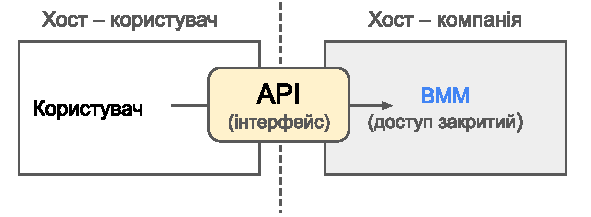
\includegraphics[width=0.8\textwidth]{closed_source_llm.pdf}
    \caption{Закриті ВММ доступні через API, внутрішні деталі яких приховані від користувача.}
    \label{fig:closed_source_llm_ua}
\end{figure}

\paragraph{Моделі з відкритим кодом}

Відкриті ВММ надають змогу отримати повний доступ до архітектури та параметрів моделі (кількість шарів, нейронів, ваги зв'язків і тд.), забезпечуючи прозорість і можливість для проведення тонкого налаштування на локальному пристрої, як це зображено на рис.~\ref{fig:open_source_llm_ua}. Для їхнього навчання або тонкого налаштування можуть знадобитися великі обчислювальні ресурси, однак за рахунок доступності та детальних описів моделей, вони нерідко є основним вибором при проведенні дослідницької роботі та експериментів.

\begin{figure}[h]
    \centering
    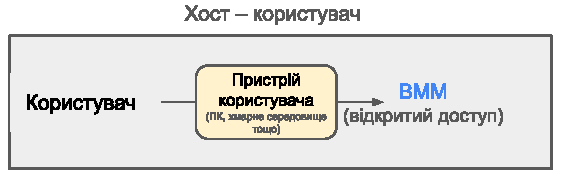
\includegraphics[width=0.8\textwidth]{open_source_llm.pdf}
    \caption{Відкриті ВММ дозволяють доступ до коду та архітектурних деталей, сприяючи локальному експериментуванню та донавчанню.}
    \label{fig:open_source_llm_ua}
\end{figure}

\subsection{Підготовка моделей для локального запуску експериментів}

Для проведення експериментів використовувалися версії моделей GPT-4 (Turbo, 4o-mini), LLaMA (2, 3, 3.1), Mixtral, Qwen (2, 2.5) -- у кількох розмірах (-7B, -8B, -13B, -70B, -8x7B, -405B) та специфікаціях (-Math, -Instruct, -Chat), які показали різні результати роботи з обробкою математичних комбінаторних задач.

Для моделей у відкритому доступі було використано їхні квантовані копії задля оптимізації використання ресурсів при локальному запуску моделей. Це дозволило зменшити обсяг необхідної пам'яті та прискорити обчислення без значної втрати точності.

Під час роботи для проведення експериментів з відкритими моделями використовувалися графічні відеокарти Nvidia Quadro RTX 8000\footnote{\url{https://www.nvidia.com/content/dam/en-zz/Solutions/design-visualization/quadro-product-literature/quadro-rtx-8000-us-nvidia-946977-r1-web.pdf}.} з 48 ГБ оперативної пам’яті та Nvidia A100\footnote{\url{https://www.nvidia.com/content/dam/en-zz/Solutions/Data-Center/a100/pdf/nvidia-a100-datasheet-us-nvidia-1758950-r4-web.pdf}.} з 80 ГБ оперативної пам’яті. Хоча пам'ять не була повністю зайнята під час експериментального процесу, видно, що GPU-Util була завантажена на 100\% (Рисунок \ref{fig:gpu_util}), що свідчить про ``вузьке місце'' обробки даних під час виконання кількох екземплярів ВММ локально на одному GPU.

Задля оптимізації та більш ефективної роботи відеокарти та створення ефективного процесу роботи з даними рекомендується використовувати кілька окремих графічних карт та об'єднувати у спільну мережу, наприклад, за допомогою технології PARCS-JAVA \cite{Anisimov2005}, які можуть дозволити проведення роботи систем без перевантаження Util-процесів.

Крім цього, результати досліджень, які представлені у статті \cite{vlasenko2019methodology}, доводять, що використання методики визначення опорної матриці моніторингу домену управління дозволяє оптимізувати інтервали опитування мережевих елементів. Зокрема, завдяки побудові дерева мережі з використанням теорії графів та методу послідовного зменшення невідомих для розв’язання системи лінійних нерівностей було можливе визначення мінімальних значень періодів моніторингу, які запобігають перевантаженню мережі службовим трафіком. Інтеграція цих підходів до експериментальної частини дослідження сприяла більш ефективному розподілу навантаження на графічну карту та оптимізації використання апаратних ресурсів.

\begin{figure}
    \centering
    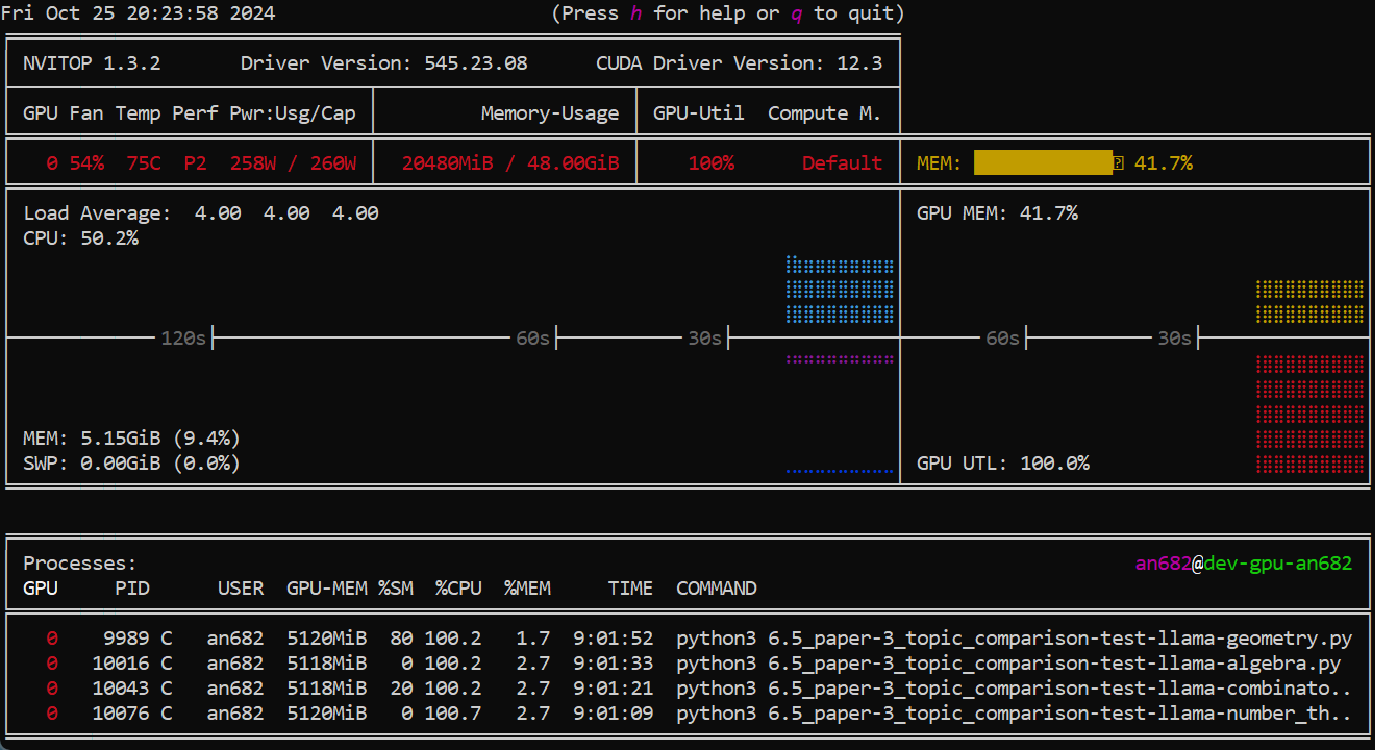
\includegraphics[width=0.9\textwidth]{data/gpu_util.pdf}
    \caption{Кілька процесів, що виконуються на графічній відеокарті, але завантажують роботу процесора на 100\%, чим сповільнюють швидкість виконання обчислень.}
    \label{fig:gpu_util}
\end{figure}

\subsection{Використання API}

Для роботи з закритими моделями використовується прикладний програмний інтерфейс (API, Application Programming Interface).

У експерименті використовувалися закриті моделі \texttt{GPT-4-Turbo-preview-v1106} та \texttt{GPT-4o-mini-2024-07-18}, які завдяки API дозволяють налаштовувати параметри без необхідності локального розгортання. 

Це забезпечує зручний інтерфейс для інтеграції моделей в експериментальне середовище.

Для проведення експерименту з \texttt{LLaMA-3.1-405B-Instruct} використовувалася також відкрита ВММ LLaMA 3.1 \cite{grattafiori2024llama3herdmodels}, яка містить близько 405 млрд. параметрів. Оскільки ця модель вимагає значної кількості додаткової пам’яті для роботи, задля запуску моделі та обробки запитів було використано хмарний сервіс Lepton AI\footnote{\url{https://www.lepton.ai/}.}, на якому відповідна модель зберігалася у квантованому вигляді.

Повний перелік моделей, використаних у експериментальній частині дослідження, наведено в Додатку~\fullref{sec:models-tested}.

\subsection{Приклад завантаження мовної моделі}

Робота з ВММ передбачає вибір та розгортання відповідних моделей. Ресурс Hugging Face\footnote{\url{https://huggingface.co/}.} є одним з найбільш поширених ресурсів для завантаження різноманітних ВММ. При виборі моделей слід звернути увагу на необхідну кількість оперативної пом'яти для роботи з моделлю. Багато моделей представлені на ресурсі мають їхні квантовані версії, які потребують менше оперативної пам'яті для роботи з ними. Наприклад, мовна модель LLaMA-3.1-8B, яка має близько 8 млрд параметрів, у 16-бітному вигляді потребує 16 ГБ оперативної пам'яті для виведення результатів, тоді як 8-бітна квантована версія -- лише 8 ГБ, але матиме меншу точність. Детальніше про квантування моделей у наступному розділі~\fullref{sec:quatisation}).

Нижче наведено фрагмент коду мовою Python для запуску та виконання запитів з моделлю LLaMA-2-70b-Chat (квант. GGUF) на віртуальній машині:
\begin{lstlisting}[language=python, breaklines=true]
#!/bin/python
import os
import sys
from termcolor import colored
from llama_cpp import Llama

MODEL_PATH = "models/llama-2-70b-chat.Q4_K_M.gguf"

MAX_TOKENS = 2048

def run_console_app():
    if not os.path.isfile(MODEL_PATH):
        print(f"Error: Invalid model path '{MODEL_PATH}'")
        sys.exit(1)

    llm = Llama(model_path=MODEL_PATH, n_gpu_layers=-1)

    print(colored("\n## Welcome to the Llama Console App! ##\n", "yellow"))
    print("Enter your prompt (or 'q' to quit):")

    while True:
        user_input = input("> ")
        if user_input.lower() == 'q':
            print("Exiting...")
            break

        user_input = f"Q: {user_input} A:"
        print(colored("Processing...", "yellow"))

        try:
            output = llm(user_input, max_tokens=MAX_TOKENS, stop=["Q:"], echo=True)

            choices_text = output["choices"][0]["text"]
            choices_text = choices_text.replace(user_input, "").strip()
            formatted_text = colored(choices_text, "green")
            print(f"\n{formatted_text}\n")
        except Exception as e:
            print(f"Error: Failed to generate response. {str(e)}")

if __name__ == '__main__':
    run_console_app()
\end{lstlisting}

Приклад вихідного тексту:
\begin{lstlisting}[language=JSON, breaklines=true]
   {"content":  Solve the following mathematical problem:
                You have 3 green apples and 5 red apples.
                How many green objects do you have?}
\end{lstlisting}


%%%%%%%%%%%%%%%%%%%%%%%%%%%%%%%%%%%%%%%%%%%%
\section{Квантування моделей}
\label{sec:quatisation}

Зі зростанням популярності інтелектуальних мобільних пристроїв та високими обчислювальними витратами моделей на базі нейронних мереж, з’явилася нагальна потреба в ефективних і точних схемах взаємодії з такими моделями безпосередньо на кінцевому пристрої. Одним зі способів розв’язання цієї проблеми є \emph{квантування моделей} -- техніка, що дає змогу зменшити обчислювальні витрати та споживання пам’яті завдяки переходу на низькорозрядні типи даних.

\subsection{Теоретичні відомості процесу квантування}

Ідея квантування полягає у стисканні моделей таким чином, аби можна було виконувати обчислення з меншими витратами ресурсів, за потреби з використанням виключно цілочисельної арифметики. Така оптимізація особливо корисна, коли апаратне забезпечення (наприклад, мобільні процесори чи мікроконтролери) не мають вбудованих реалізації для виконання числових операцій для чисел з рухомою комою.

Загалом квантування дозволяє (1) суттєво зменшити використання пам’яті моделі, (2) збільшити швидкість обчислень і (3) зберегти корисний рівень ефективності моделі. У результаті застосування низькорозрядних типів, наприклад \texttt{int8} або \texttt{float16}, на практиці можна досягнути більш економного виведення результатів при наближенні точності до початкової.

У квантованих моделях часто спостерігається зростання розрідженості, про яку згадувалося раніше, коли значна кількість параметрів може бути перетворена на нуль. Відповідно з’являється можливість додатково пришвидшити обчислення, не оброблюючи нулеві значення.

\paragraph{Наївне квантування та метод K-means}

Для демонстрації ключових підходів квантування варто розглянути два методи. \emph{Наївне квантування (Naive quantisation)} рівномірно знижує точність усіх параметрів, що можна уявити як розбиття простору на рівні за розміром ``клітинки''. Таке ділення не є рівномірним за кількістю відповідних елементів моделі, та в окремих ділянках може призвести до втрати інформації.

Натомість \emph{K-means квантування (K-means quantisation)} виконує поділ на кластери відповідно до фактичного розташування точок, забезпечуючи точніше представлення значень. Кожній точці (вазі) призначається найближчий центроїд у просторі. Завдяки цьому можна краще зберегти основні параметри моделі.

Приклад різниці між даними підходами показано на рис.~\ref{fig:quantisation}.

\begin{figure}[h]
    \centering
    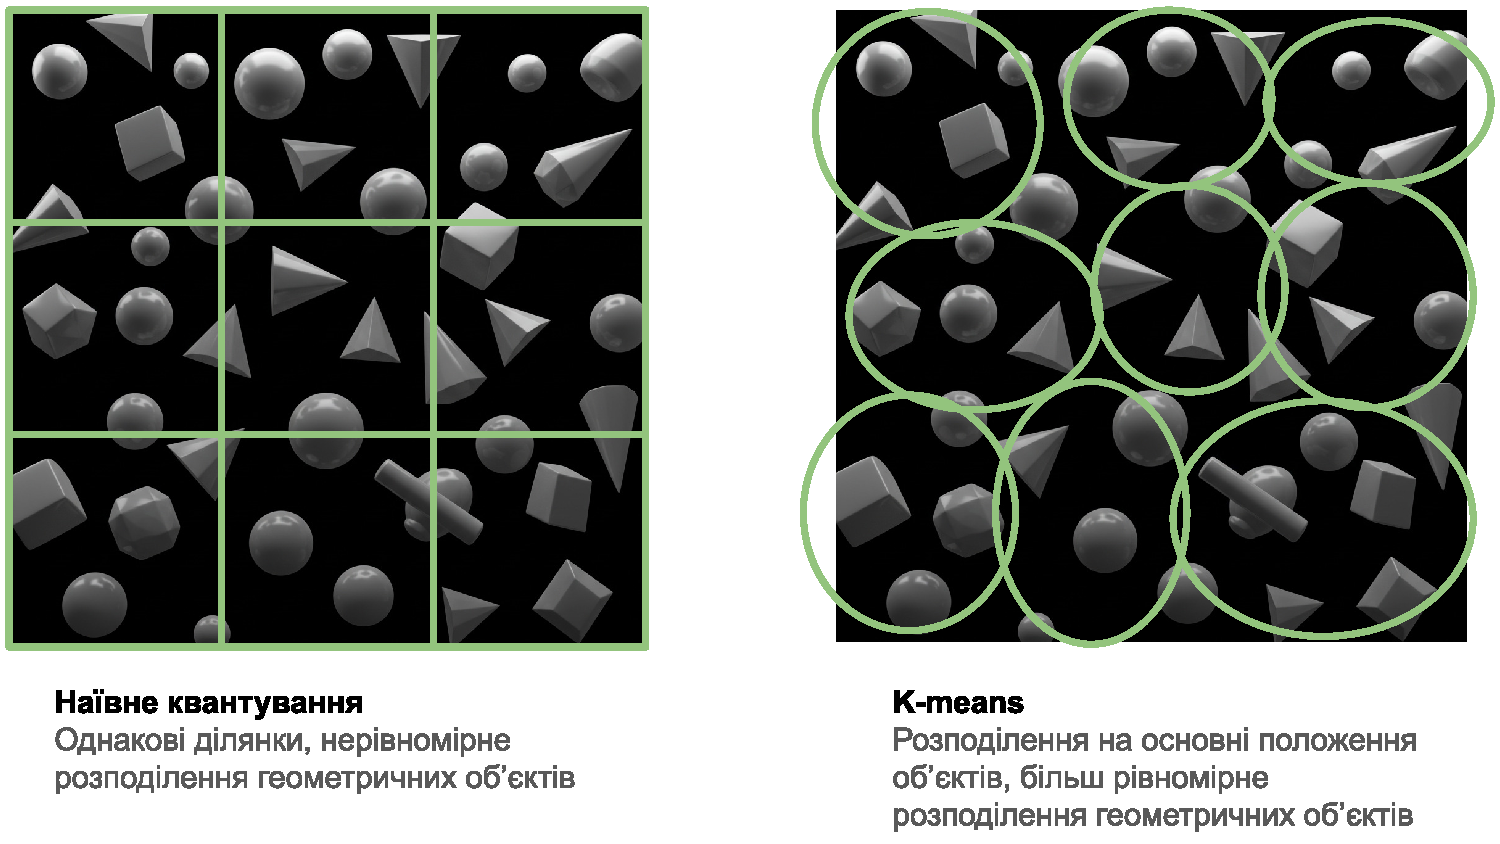
\includegraphics[width=0.8\textwidth]{quantisation_example.pdf}
    \caption{Схематичне відображення відмінностей між наївним квантуванням (ліворуч) та квантуванням за допомогою K-means (праворуч).}
    \label{fig:quantisation}
\end{figure}

\subsection{Квантування при роботі з типами даних}

Квантування зазвичай супроводжується переходом від \texttt{float32} до форматів нижчої розрядності, наприклад \texttt{float16}, \texttt{bfloat16}, \texttt{int8} тощо. Зниження числа бітів зменшує пам’ять для зберігання та спрощує обчислення. Водночас для операцій на кшталт множення потрібно мати тип накопичення з більшою розрядністю (\texttt{int32}, \texttt{float32}), щоб уникнути надто грубого заокруглення значень.

Одним з прикладів переходу є \texttt{float32} $\rightarrow$ \texttt{float16}. Ці формати є сумісними за схемою числа з рухомою комою, але \texttt{float16} має менший динамічний діапазон і може спричинити до проблем з обчисленнями занадто малих або занадто великих чисел. Проте для більшості обчислень у нейронних мережах цього діапазону достатньо.

Складнішим є перехід \texttt{float32} $\rightarrow$ \texttt{int8}, де відображення відбувається в дискретний простір, що охоплює лише 256 значень. Для цього часто використовують \emph{афінне квантування (affine quatisation)}:
\begin{equation}
x = S \cdot (x_q - Z).
\end{equation}

Тут $x$ -- початкове (floating) значення, $x_q$ -- квантоване \texttt{int8}, а $S$ і $Z$ відповідають за масштаб і нульову точку. Процес супроводжується заокругленням:
\begin{equation}
x_q = \text{round}\!\bigl(x/S + Z\bigr),
\end{equation}

та, за потреби, обрізанням вхідних значень, що виходять за встановлений діапазон. Кілька деталей стосовно навчання моделей після квантування описано у роботі~\cite{jacob2017quantizationtrainingneuralnetworks}.

\paragraph{Квантування за допомогою методу K-means}

У багатьох експериментальних задачах, зокрема для відкритих мовних моделей, використовують \emph{K-means Quantisation} з бібліотекою \texttt{llama.cpp}. Завдяки такому підходу, моделі ефективніше зберігають свої можливості й можуть набагато швидше працювати локально на звичайних пристроях. Наприклад, при квантуванні за допомогою \texttt{llama.cpp} тип квантування Q4\_K\_M значить:
\begin{itemize}
    \item {Q} -- квантування (Quantisation),
    \item {4} -- використання 4 біт на параметр,
    \item {K} -- кластеризація параметрів методом K-means,
    \item {M} -- розмір моделі після квантування (наприклад, Medium).
\end{itemize}

\subsection{Формат GGUF}

Квантовані версії моделей зберігаються у окремому файлі. Одним з поширених на даний момент форматів з є \emph{GGUF} (Generic GPT Unified Format). Раніше нейронні мережі зберігали у широковживаних форматах \texttt{.pb} для TensorFlow, \texttt{.pt} / \texttt{.pth} для PyTorch, \texttt{ONNX} для обміну між фреймворками, однак вони зазвичай: (1) зберігали повну точність \texttt{float32}, (2) не були зосереджені на квантуванні та (3) не враховували специфіки великих мовних моделей.

Поява формату GGML стала першим кроком у напрямку зниження точності до \texttt{int8} чи \texttt{int4}, що відчутно скоротило розміри файлу і надало можливість запуску великих моделей на кінцевих пристроях. Формат GGUF продовжив цей напрямок, але додав ширші можливості з управління метаданими, підтримку більших моделей (понад 100 ГБ у розмірі) і поліпшений опис архітектури.

Зокрема, GGUF призначений для генеративних моделей зі значною кількістю параметрів. Він дає змогу задати різні рівні квантування (4-біт, 8-біт тощо) і зберігати детальнішу інформацію моделі (параметри квантування, архітектуру, схему токенізації). З погляду виведення результатів це робить запуск моделей більш ефективним, оскільки всі потрібні метадані вбудовані безпосередньо у структуру файлу. Приклад структури файлу у форматі GGUF зображено на рис.~\ref{fig:gguf_architecture}.

\begin{figure}[h]
    \centering
    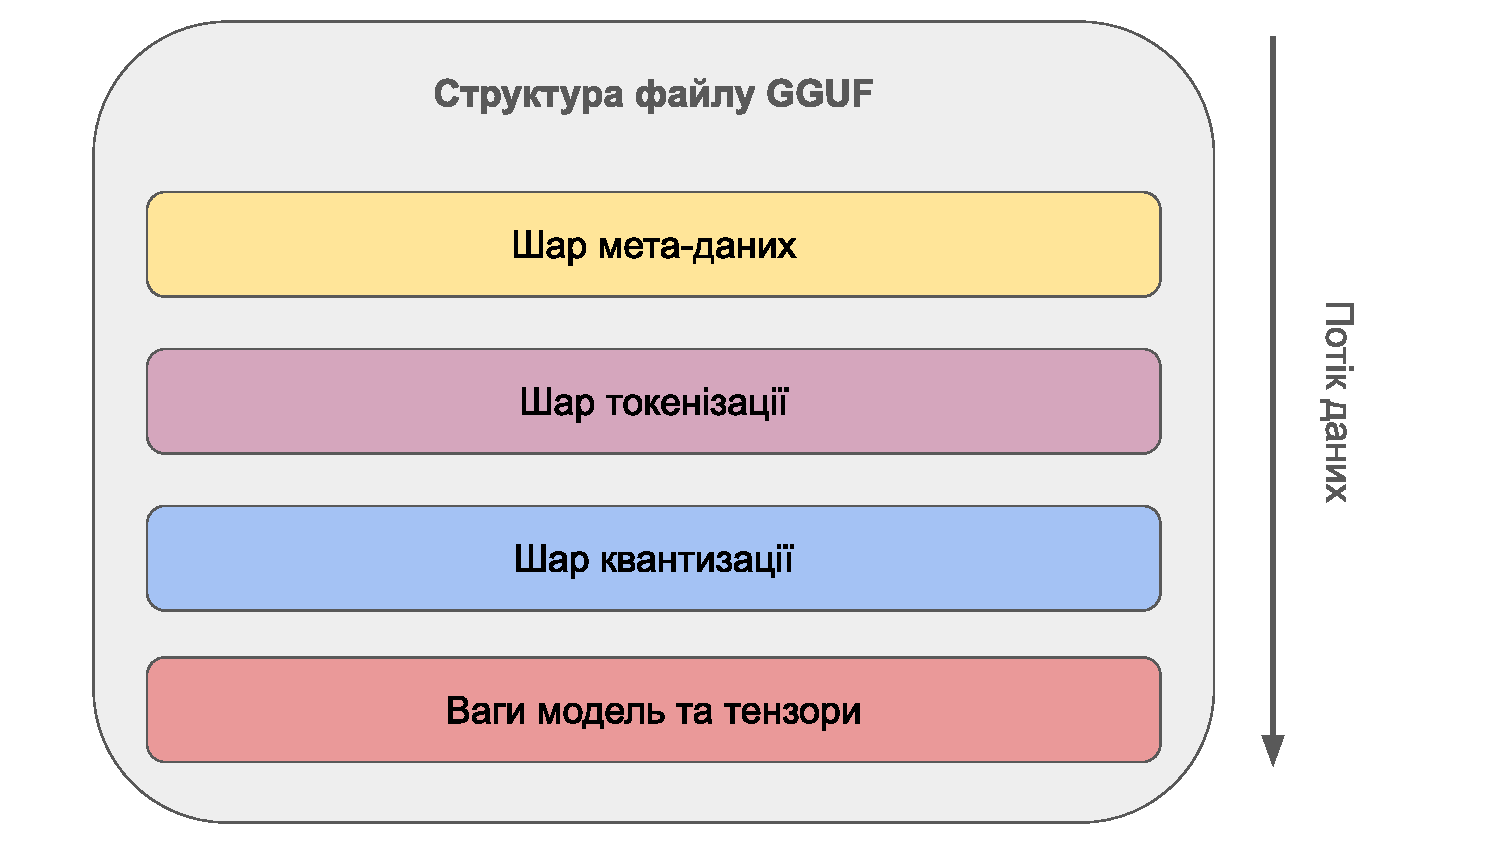
\includegraphics[width=0.8\textwidth]{gguf_architecture.pdf}
    \caption{Приклад структури файлу у форматі GGUF (умовне ілюстративне зображення).}
    \label{fig:gguf_architecture}
\end{figure}

На практиці застосування 4-бітної квантизації у форматі GGUF дає змогу знизити вимоги до оперативної пам’яті більш ніж утричі. Наприклад, для моделі LLaMA-3.1-8B зменшуючи її обсяг із 16 ГБ до приблизно 4.5 ГБ. Це дозволяє запускати більші моделі на пристроях із обмеженими ресурсами. Щодо швидкодії, залежно від конкретної реалізації та апаратного забезпечення, швидкість генерації тексту відповідно може пришвидшитися у 2-3 рази. Завдяки цим вдосконаленням великі моделі можна ефективно використовувати на пристроях з обмеженими обчислювальними ресурсами (edge-AI, мобільні системи), а також у середовищах, де є потреба в економному розподілі обладнання.

Таким чином, квантування моделей -- важливий інструмент оптимізації сучасних мовних моделей. Методи на кшталт наївного квантування, K-means квантованих схем і використання низькорозрядних типів (\texttt{float16}, \texttt{int8}, \texttt{int4}) допомагають суттєво зменшити розмір і прискорити роботу моделей із незначними втратами в точності. Формати GGML та GGUF, які є поширеними у спільноті дослідників, демонструють, як можна системно впровадити квантування і зробити великі мовні моделі більш доступними та гнучкими для різноманітних застосунків.

\subsection{Характеристики моделей використаних у експериментуванні}
\label{sec:models-tested}

У таблиці~\ref{tab:models-tested} представлено детальний перелік моделей, використаних у експериментальній частині дослідження. Усі моделі об'єднані у спільну таблицю для зручного порівняння їхніх характеристик.

\begin{figure}[!ht]
    \captionof{table}{Специфікації моделей, використаних у експерименті.}
    \label{tab:models-tested}
    \renewcommand{\arraystretch}{1.2}
    \resizebox{\textwidth}{!}{%
    \begin{tabular}{|c|l|c|c|c|p{2.5cm}|p{3cm}|l|l|}
        \hline
        \textbf{no.} & \textbf{Модель} & \textbf{Параметри} & \textbf{Кв.} & \textbf{Метод квант.} & \textbf{Довж. конт. вікна} & \textbf{Дата оновлення знань} & \textbf{Доступ} & \textbf{Розробник} \\ \hline

        1 & LLaMA-2-7B-Chat & 7 млрд & \ding{51} & Q4\_K\_M & 4k & Липень 2023 & Відкритий код & Meta \\ \hline

        2 & LLaMA-2-13B-Chat & 13 млрд & \ding{51} & Q4\_K\_M & 4k & Липень 2023 & Відкритий код & Meta \\ \hline
                
        3 & LLaMA-2-70B-Chat & 70 млрд & \ding{51} & Q4\_K\_M & 4k & Липень 2023 & Відкритий код & Meta \\ \hline

        4 & Llama-3-8B-Instruct & 8 млрд & \ding{51} & Q4\_K\_M & 128k & Грудень 2023 & Відкритий код & Meta \\ \hline
        
        5 & LLaMA-3.1-70B-Instruct & 70.6 млрд & \ding{51} & Q4\_K\_M & 128k & Грудень 2023 & Відкритий код & Meta \\ \hline

        6 & LLaMA-3.1-405B-Instruct & 405 млрд & \ding{55} & н/д & 128k & Грудень 2023 & API & Meta \\ \hline

        7 & Mixtral-8x7B & 56 млрд & \ding{51} & Q4\_K\_M & 32k & н/д & Відкритий код & Mistral AI \\ \hline  
                        
        8 & Mixtral-8x7B-Instruct & 56 млрд & \ding{51} & Q4\_K\_M & 32k & н/д & Відкритий код & Mistral AI \\ \hline

        9 & Mathstral-7B & 7.25 млрд & \ding{51} & Q4\_K\_M & 32k & н/д & Відкритий код & Mistral AI \\ \hline
        
        10 & Qwen2-7B-Instruct & 7 млрд & \ding{51} & Q4\_K\_M & 128k & н/д & Відкритий код & Alibaba Cloud \\ \hline
        
        11 & Qwen2-Math-7B & 7 млрд & \ding{51} & Q4\_K\_M & 128k & н/д & Відкритий код & Alibaba Cloud \\ \hline

        12 & Qwen2.5-Math-7B & 7.62 млрд & \ding{51} & Q4\_K\_M & 128k & н/д & Відкритий код & Alibaba Cloud \\ \hline

        13 & GPT-4-Turbo-preview-v1106 & н/д & \ding{55} & н/д & 128k & Квітень 2023 & API & OpenAI \\ \hline
        
        14 & GPT-4o-mini-2024-07-18 & н/д & \ding{55} & н/д & 128k & Жовтень 2023 & API & OpenAI \\ \hline
        
    \end{tabular}%
    }
\end{figure}

Детальний опис моделей та відповідні файли квантованих версії можна знайти у Додатку~\fullref{sec:models-tested-links}.

%%%%%%%%%%%%%%%%%%%%%%%%%%%%%%%%%%%%%%%%%%%%
\section{Тестування моделей задачами з різних математичних розділів}

Було досліджено ефективність моделей у розв'язанні задач з наступних математичних розділів: алгебра, геометрія, теорія чисел, комбінаторика. Було відібрано 8,000 задач з початкового набору даних NuminaMath-TIR \cite{numina_math_7b}, який містить 72,540 задач та проведено аналіз точності моделей у кожному розділі згідно методу описаного у роботі \cite{nikolaiev2024comparison}. 

Для проведення тестування були використані відкриті моделі Llama-3.1-8B-Instruct, Qwen2.5-Math-7B, Mathstral-7B та закрита модель GPT-4o-mini. Обчислення виконувалися на графічній відеокарті Nvidia Quadro RTX 8000. Результати експерименту описані у наступному розділі дисертаційної роботи.

\section{Тестування моделей на власному наборі задач}

\subsection{Комп'ютерні ресурси для обчислення}

У лаштунках наукової роботи було проведено експериментальне дослідження здатності моделей розв'язувати комбінаторні задачі з лінгвістичними та структурними змінами в умовах задач. Було виконано порівняння роботи моделей GPT-4, LLaMA (версії 2 та 3.1), Mixtral, які потім було порівняно з результатами людей-експертів \cite{nikolaiev2024can}.

У таблиці~\ref{tab:llm_computation} наведено загальний обсяг оброблених запитів та час на обробку. Тестування відбувалося у три серії, які виконувалися з оновленою версією набору даних та відповідних моделей кожна з яких відділена подвійною лінію у таблиці ~\ref{tab:llm_computation}.

Тестування моделей виконувалося у вигляді звичайного запиту у вигляді задачі разом з додатковою інструкцією або лише задачі без додаткової інструкції. Загальна кількість запитів склала близько 30 тис. на експериментальних серіях 1-2 та ще 6 тис. на третій серії експериментів, разом -- близько 36 тис. запитів. Кожен запит ініціювався у вигляді окремого діалогу з моделлю. На обчислення за допомогою GPU RTX8000, A100, а також ресурсів від Open AI було витрачено разом близько 225 годин роботи моделей. Виконання запитів Open AI виконувалося швидко, з приблизною вартістю близько \$12.60 за 1375 одиниць запитів (з урахуванням попереднього тестування).

\begin{figure}[!ht]
    \centering
    \captionof{table}{Результати експериментів з ВММ.  
    Види варіацій: A = звичайна, B = математична, C = надлишкова, D = параметризована, E = лінгвістичне заплутування.}  
    \label{tab:llm_computation}
    \renewcommand{\arraystretch}{1.2}
    \resizebox{\textwidth}{!}{%
    \begin{tabular}{|l|l|c|c|c|c|c|c|l|}
    \hline
    \multirow{2}{*}{\textbf{Модель}} & \multirow{2}{*}{\textbf{Додаткова інструкція (англ.)}} & \multicolumn{5}{c|}{\textbf{Варіації задач}} & \multirow{2}{*}{\textbf{Час оброб.}} & \multirow{2}{*}{\textbf{GPU}} \\
    \cline{3-7}
    & & A & B & C & D & E &  &  \\
    \hline
    \hline

    LLaMA-2-7B/13B/70B & <None> & $25 \times 10$ & $25 \times 10$ & - & - & $25 \times 10$ & 10 год & RTX8000 \\
    LLaMA-2-7B/13B/70B & Give a short answer. & $25 \times 10$ & $25 \times 10$ & - & - & $25 \times 10$ & 10 год & RTX8000 \\
    LLaMA-2-7B/13B/70B & The answer is & $25 \times 10$ & $25 \times 10$ & - & - & $25 \times 10$ & 10 год & RTX8000 \\
    LLaMA-2-7B/13B/70B & The answer (arabic numerals) is & $25 \times 10$ & $25 \times 10$ & - & - & $25 \times 10$ & 10 год & RTX8000 \\
    LLaMA-2-7B/13B/70B &  Let’s think step by step. & $25 \times 10$ & $25 \times 10$ & - & - & $25 \times 10$ & 10 год & RTX8000 \\
    \hline
    \hline

    LLaMA-2-7B/13B/70B & <None> & $25 \times 10$ & $25 \times 10$ & $25 \times 10$ & $25 \times 10$ & $25 \times 10$ & 27.5 год & RTX8000 \\
    LLaMA-2-7B/13B/70B &  The short and correct answer. & $25 \times 10$ & $25 \times 10$ & $25 \times 10$ & $25 \times 10$ & $25 \times 10$ & 28.5 год & RTX8000 \\
    LLaMA-2-7B/13B/70B &  Give me a short expression as an answer. & $25 \times 10$ & $25 \times 10$ & $25 \times 10$ & $25 \times 10$ & $25 \times 10$ & 28 год & RTX8000 \\
    \hline
    Mixtral-8x7B-/Instruct & <None> & $25 \times 10$ & $25 \times 10$ & $25 \times 10$ & $25 \times 10$ & $25 \times 10$ & 12.5 год & RTX8000 \\
    Mixtral-8x7B-/Instruct & The short and correct answer. & $25 \times 10$ & $25 \times 10$ & $25 \times 10$ & $25 \times 10$ & $25 \times 10$ & 9.5 год & A100 \\
    Mixtral-8x7B-/Instruct & The short and correct answer. & $25 \times 10$ & $25 \times 10$ & $25 \times 10$ & $25 \times 10$ & $25 \times 10$ & 12.5 год & RTX8000 \\
    \hline
    \hline

    LLaMA-3.1-70B-Instruct & <None> & $25 \times 10$ & $25 \times 10$ & $25 \times 10$ & $25 \times 10$ & $25 \times 10$ & 15 год & RTX8000 \\
    LLaMA-3.1-70B-Instruct & The short and correct answer is & $25 \times 10$ & $25 \times 10$ & $25 \times 10$ & $25 \times 10$ & $25 \times 10$ & 15 год & RTX8000 \\
    \hline
    Mixtral-8x7B-Instruct & <None> & $25 \times 10$ & $25 \times 10$ & $25 \times 10$ & $25 \times 10$ & $25 \times 10$ & 12.5 год & RTX8000 \\
    Mixtral-8x7B-Instruct & The short and correct answer is & $25 \times 10$ & $25 \times 10$ & $25 \times 10$ & $25 \times 10$ & $25 \times 10$ & 12.5 год & RTX8000 \\
    \hline
    GPT-4-Turbo & <None> & $25 \times 5$ & $25 \times 5$ & $25 \times 5$ & $25 \times 5$ & $25 \times 5$ & 1-2 год & API \\
    GPT-4-Turbo & The short and correct answer is & $25 \times 5$ & $25 \times 5$ & $25 \times 5$ & $25 \times 5$ & $25 \times 5$ & 1-2 год & API \\
    \hline
    \hline
    
    \multicolumn{2}{|r|}{\textbf{Загально:}} & \multicolumn{5}{|r|}{\textbf{36,250 запитів}} & \textbf{225.5 год} & - \\
    \hline
    \end{tabular}%
    }
\end{figure}

\subsection{Критерії оцінювання відповідей моделей}

Задля перевірки результатів роботи моделей було розроблено критерії оцінювання, які враховують точність, повноту та логічну послідовність наведених розв'язань. Це забезпечує об'єктивність та порівнянність результатів між різними моделями та з результатами людей. Схема включає бінарну оцінку правильності розв'язків та аналіз проміжних кроків генерації розв'язання.

Це досягається за рахунок набору правил, які застосовувалася для надання оцінок відповідям моделей. Оскільки експериментування відбувалося з математичними комбінаторними задачами, у деяких випадках люди та ВММ повертають відповіді не у числовій формі, а як комбінаторну формулу з використанням біномів, факторіалів та інших комбінаторних символьних представлень, наприклад, відповіді у вигляді \(C(11, 2) = 55\) -- також приймалися, якщо вони еквіваленті числовому значенню правильної відповіді на задачу. Нижче перелічено набір правил, які були застосовані у схемі оцінювання, включаючи випадки ``сірої зони'', коли відповідь моделі можна трактувати по-різному. Критерії оцінювання наведені нижче.

Критерії оцінювання за надання ``1'' (розв'язок правильний):
\begin{enumerate}
    \item \textit{Бал: 1} -- Відповідь коротка та правильна.
    \item \textit{Бал: 1} -- На початку наведенo правильний розв'язок, навіть якщо далі слідує неправильна або нерелевантна інформація.
    \item \textit{Бал: 1} -- Наприкінці наведено правильний розв'язок, навіть якщо перед цим присутня неправильна або нерелевантна інформація.
    \item \textit{Бал: 1} -- Модель перелічує кілька варіантів розв'язку та вказує на правильний.
    \item \textit{Бал: 1} -- Модель починає з неправильного розв'язку, але потім приходить до правильного.
    \item \textit{Бал: 1} -- Комбінаторний розв'язок правильний, але модель надає наближену числову відповідь (наприклад, з використанням слів ``приблизно'', ``близько'', символу ``\(\approx\)'' тощо).
\end{enumerate}

Критерії оцінювання за надання ``0'' (розв'язок неправильний):
\begin{enumerate}
    \item \textit{Бал: 0} -- Розв'язок неправильний.
    \item \textit{Бал: 0} -- Розв'язок відсутній.
    \item \textit{Бал: 0} -- Розв'язок не містить числових або комбінаторних елементів.
    \item \textit{Бал: 0} -- Модель не завершила розв'язання та не прийшла до фінального розв'язку.
    \item \textit{Бал: 0} -- Модель перелічує кілька розв'язків (можливо, разом з правильним), але обирає неправильний або жодний.
    \item \textit{Бал: 0} -- Розв'язок був представлений у вигляді мовою програмування.
    \item \textit{Бал: 0} -- Модель має правильні кроки обґрунтування, але приходить до неправильного висновку.
    \item \textit{Бал: 0} -- Модель виконала неправильний перехід під час обрахунків; відповіді частини перетворень з'єднані знаком рівності або такими, як наприклад, ``або'', ``дорівнює'' тощо.
    \item \textit{Бал: 0} -- Розв'язок неоднозначний (не надано фінальної розв'язку).
\end{enumerate}

Схема оцінювання забезпечує детальну та об'єктивну оцінку відповідей моделей, враховуючи різні формати відповідей та можливі варіанти їх подання. Це дозволяє точно визначити правильність розв'язку, навіть якщо він представлений у незвичайній формі. Крім того, врахування ``сірої зони'' дозволяє більш гнучко перевіряти відповіді моделей, які є частково правильними або потребують додаткової інтерпретації.

\section{Генерація синтетичних варіацій комбінаторних задач}

Задля генерації задач було використано підхід описаний у роботі \cite{nikolaiev2025synth} з фінальним набором, що містив 1,000 комбінаторних задач. Даний набір даних був розширений до 5,583 задач за допомогою методів відбору даних описаних у відповідній роботі. Нижче описується послідовність кроків, які були виконані для проведення експериментальної частини дослідження з відповідними даними.

Задля проведення експериментальної частини було використано набір даних Numina-CoT \cite{numina_math_7b}, який як згадувалися раніше, містить близько 860 тис. різноманітних математичних задач.

\subsection{Генерація синтетичних варіацій задач}

Генерація синтетичних даних включає систематичну маніпуляцію з текстовими умовами задач відфільтрованого набору даних. В результаті вводиться кілька нових варіацій задач: (i) \emph{художня варіація} з заміною стилю тексту задачі у вигляді вигаданої історії; (ii) \emph{надлишкова варіація}, у який вводиться зайва числова інформація у формулювання оригінальної умови задачі; та (iii) \emph{прихована варіація}, що розміщує задачу у нерелевантному контексті. Аналогічно до переднього етапу, задля вищої точності роботи з моделями, а також оскільки вхідні дані задані англійською мовою, усі інструкції передавалися до моделей англійською мовою.

Процес генерації варіацій текстів задач відбувається на основі оригінального тексту задач за допомогою ВММ GPT-4o-mini. Модель було обрано завдяки її швидкості та ефективності роботи з технічними текстами, зокрема з темами з математики, програмування та питаннями пов'язанні із наукою. Вона призначена для вирішення складних завдань, але при цьому є ресурсоефективною, що робить її придатною для обробки великого набору даних. Модель має контекстне вікно у розмірі 128,000 токенів і зріз знань на момент жовтня 2023 року\footnote{\url{https://openai.com/index/gpt-4o-mini-advancing-cost-efficient-intelligence/}}.

Звернення до моделі відбувалися за допомогою API. У відповідному запиті до моделі було додано інструкцію про те, щоб варіації задачі зберігали математичну основу задля забезпечення однакового числового розв'язку, що є важливим для подальшого оцінювання точності згенерованих даних. Додатково у запитах до моделі було внесено інструкцію про збереження розміру варіацій задач подібним до оригіналу, але в багатьох випадках з художньою варіацією модель порушувала дану умову, що приводило до генерації більш довгих текстів задач. Середня довжина (у кількості символів) згенерованих текстів варіації задач зазначено у таблиці~\ref{tab:var_len}.

\begin{figure}
    \centering
    \captionof{table}{Середня довжина умов варіацій задач.}
    \label{tab:var_len}
    \begin{tabular}{|l|c|}
    \hline
    Варіація & Сер. к-ть символів \\
    \hline
     Оригінальна & 248 \\
     Художня & 651 \\
     Надлишкова & 303 \\
     Прихована & 320 \\
     \hline
    \end{tabular}
\end{figure}

Процес генерації синтетичних версій задач на основі оригінальних текстів виконувався за наступним запитом, де за допомогою параметру style було задано відповідну варіацію задачі:

\begin{lstlisting}[language=json, breaklines=true]
{"content": "Apply the {style} to the following mathematical 
            problem. Retain the mathematical core and keep
            the resulting statement approximately similar 
            in length. Return just the problem statement. 
            Problem: {problem_statement}"}
\end{lstlisting}

\subsection{Генерація розв'язків}

Щоб забезпечити якість міркування і покращити точність моделі у розв'язанні задач, виконувалося 2 етапи:

\begin{enumerate}
    \item Модель GPT-4o-mini використовується для розв'язання усіх варіацій задач. Для кожної варіації задачі разом з оригінальним формулюванням умови, було згенеровано математичне розв'язання за наступним запитом:
\begin{lstlisting}[language=json, breaklines=true]
{"content": "Solve the following mathematical problem. 
            Return a solution with the final numerical 
            answer at the end. Problem: 
            {problem_statement}"}
\end{lstlisting}
    
    \item Після цього зі згенерованого розв'язання вилучається числова відповідь (розв'язок). Для вилучення відповідей використовується нейромережевий метод, описаний у Розділі~\fullref{sec:problem-selection}. У деяких випадках мовна модель не змогла згенерувати розв'язання з єдиною позитивною числовою відповіддю -- у такому разі вважається, що задачу не було розв'язано моделлю.
\end{enumerate}

Таким чином, забезпечується стабільність роботи моделі з різними варіаціями задач, тоді як етап відбору та підготовки даних відбувається незалежно та виконується іншою моделлю.

\begin{figure}[!ht]
    \small
    \centering
    \captionof{table}{Детальний опис набору даних задач та їх згенерованих синтетичних варіацій.}
    \label{tab:dataset_final}
    \begin{tabular}{|p{4.5cm}|p{9cm}|}
        \hline
        \textbf{Назва поля (початкові дані з набору Numina-CoT)} & \textbf{Оригінальна задача} \\ \hline
        \texttt{problem\_id} & Унікальний ідентифікатор для кожної задачі. \\ \hline
        \texttt{source} & Джерело задачі. \\ \hline
        \texttt{problem} & Умова задачі. \\ \hline
        \texttt{solution} & Розв'язання задачі. \\ \hline
        \texttt{messages} & Дані у форматі ланцюжка думок. \\ \hline
        \texttt{answer} & Вилучений розв'язок на задачу. \\ \hline \hline
        \textbf{(згенеровані синтетичні дані)} & \textbf{Згенеровані синтетичні дані} \\ \hline
        \texttt{fictional} & Художня варіація задачі. \\ \hline
        \texttt{adversarial} & Надлишкова варіація задачі. \\ \hline
        \texttt{contdis} & Прихована варіація задачі. \\ \hline
        \texttt{original\_sol} & Розв'язання оригінальної варіації. \\ \hline
        \texttt{fictional\_sol} & Розв'язання художньої варіації. \\ \hline
        \texttt{adversarial\_sol} & Розв'язання надлишкової варіації. \\ \hline
        \texttt{contdis\_sol} & Розв'язання прихованої варіації. \\ \hline
        \texttt{original\_ans} & Вилучений розв'язок оригінальної варіації. \\ \hline
        \texttt{fictional\_ans} & Вилучений розв'язок художньої варіації. \\ \hline
        \texttt{adversarial\_ans} & Вилучений розв'язок надлишкової варіації. \\ \hline
        \texttt{contdis\_ans} & Вилучений розв'язок прихованої варіації. \\ \hline
    \end{tabular}
\end{figure}

\subsection{Структура зберігання синтетичного набору даних}

Кінцевий набір синтетичних даних містить 22,332 задач (з відібраного початкового набору 5,583 задач) об'єднані у колекції, що містять інформацію про кожну з задач: оригінальна, художня варіація, надлишкова варіація та прихована варіація. Кожна задача у колекції задач містить детальне розв'язання та кінцевий числовий розв'язок до неї. Детальний опис атрибутів до кожної колекції задач надано у таблиці~\ref{tab:dataset_final}. Структура розширеного набору даних відформатована та збережена Parquet і JSON для ефективної роботи мовою програмування Python 3.11. Приклад задачі наведено у Додатку~\fullref{sec:problems-synthetic}.

% Треба додати лінк на датасет (але спочатку його треба створити).

\subsection{Обмеження набору задач}

За рахунок того, що деякі задачі у оригінальному наборі даних дублюються, вони повторюються у отриманому комбінаторному наборі задач. Задачі не були прибрані з фінального набору даних, оскільки не зважаючи на співпадіння, їхня варіативність була іншою, тобто процес генерації приводив до унікальних версій тих самих задач, чим збагачував різноманітність синтетичного набору даних.

Також слід зазначити, що у оригінальному наборі задач Numina-CoT можливі помилки. Наприклад, для задачі із таблиці~\ref{tab:original_wrong} слідує, що відповідь на задачу 4, однак не складно перевірити, що можливих варіантів, що задовольняють умові задачі є 6 (числа $2005, 2050, 2500, 5002, 5020, 5200$). З урахуванням даного моменту слід зазначити, що згенеровані розв'язки до варіації початкової задачі могли бути неправильно оцінені на наступних етапах генерації задач.

\begin{figure}[h!]
    \centering
    \small
    \captionof{table}{Приклад задачі з оригінального набору Numina-CoT з помилковою відповіддю.}
    \label{tab:original_wrong}
    \begin{tabular}{|p{0.6\linewidth}|p{0.15\linewidth}|p{0.15\linewidth}|}
        \hline
        \textbf{Умова задачі} & \textbf{Відповідь Numina-CoT} & \textbf{Правильна відповідь} \\
        \hline
        How many different four-digit numbers can be formed by arranging the four digits in 2005? (\textit{Умова задачі українською:} Скільки різних чотирицифрових чисел можна утворити з числа 2005?) & \hlred{4 числа} & \hlgreen{6 чисел} \\
        \hline
    \end{tabular}
\end{figure}

\section{Експериментальна частина з участю людини}
\label{sec:human-experiment-set-up}

\subsection{Умови проведення експерименту}

Учасниками експерименту були українські школяри та студенти, які знайомі з темою комбінаторики та мають попередній досвід участі на математичних змаганнях. Загалом у дослідженні взяли участь 35 учасників віком від 13 до 18 років.

Експеримент організовано за допомогою латинського квадрату (Latin Square). Було сформовано 5 груп по 7 учасників в кожній групі з приблизно однаковим розподілом за середнім віком. Учасникам кожної групи було призначено один із п'яти комплектів задач. Кожен комплект містив 25 задач з рівномірно розподіленими варіаціями задач (5 задач на кожну з 5 варіацій). Задачі були перекладені з англійської на українську мову, щоб учасники могли впевнено прочитати та зрозуміти умови задачі. Кожен з учасників працював самостійно. Розподіл груп учасників та варіантів задач представлено на Рисунку~\ref{fig:packs}.

\begin{figure}
    \centering
    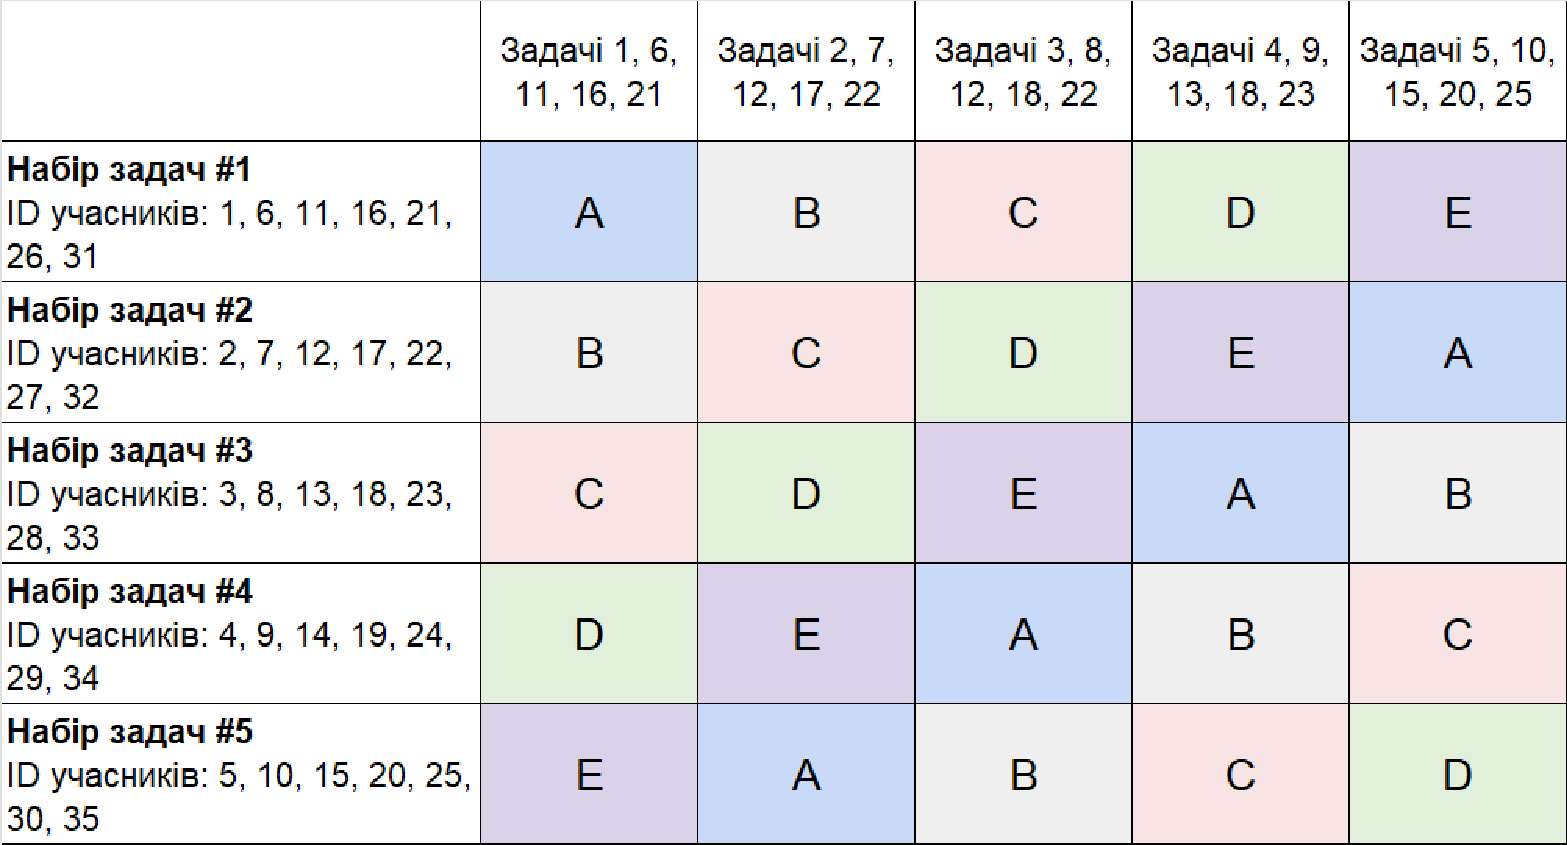
\includegraphics[width=0.8\textwidth]{packs.pdf}
    \caption{Розподіл матеріалів (задач) та учасників для проведення експериментальної частини відповідно до латинського квадрату. Букви та кольори визначають відповідні використані варіації задач: A = \hlgrey{звичайна} (сірий), B = \hlblue{математична} (блакитний), C = \hlred{надлишкова} (червоний), D = \hlgreen{параметризована} (зелений), E = \hlpurple{лінгвістичне заплутування} (фіолетовий).}
    \label{fig:packs}
\end{figure}

\subsection{Збір та підготовка даних}

Відповіді учасників були зібрані та оцінені за розробленою схемою оцінювання. Кожен учасник надавав розв'язки на задачі свого комплекту у короткій комбінаторній або числовій формі, кожен з отриманих розв'язків задач отримував оцінку 0 (неправильна) або 1 (правильна). У випадку відсутності розв'язку на певну задачу, учасник отримував оцінку 0. Враховуючи різноманітні формулювання, правильна відповідь могла бути представлена у формі комбінаторної формули, тому в деяких випадках доводилося застосовувати додаткові розрахунки під час оцінювання.

Результати між ВММ та учасниками порівнювалися наступним чином: для ВММ було обрано модель, яка продемонструвала найкращі результати роботи серед протестованих моделей, тоді як серед учасників кожної групи обиралися 5 найкращих результатів по кожній з груп, які потім разом представляли експертну оцінку.

\subsection{Умови етики для участі в експерименті}

Це дослідження було проведено як контрольований експеримент, що відбувалася відповідно до етичних стандартів залучення учасників експерименту (людей). Було залучено 35 поточних та колишніх студентів українського освітнього STEM-проекту Kvanta\footnote{\url{https://www.kvanta.xyz/}.}. Кожен учасник надав згоду з правилами участі в експерименті, для учасників молодше 16 років згоду було отримано від батьків. Експеримент оцінював математичні навички міркування на варіаціях комбінаторних задач дистанційно. Дані, які було зібрано для проведення експерименту -- вік учасників, розв'язки на переданий набір задач та час витрачений на розв'язання задач. Участь в експерименті була добровільною, і учасники були поінформовані про право відмовитися від участі в експерименті у будь-який момент. Інструкції включали загальну інформацію про кількість представлених задач, їхню складність та варіативність стилю. Грошова компенсація не передбачалася, але участь пропонувалася як навчальна можливість. Комунікація з учасниками була чіткою, підкреслюючи, що дослідження є окремим від звичайної діяльності освітнього проекту.

\subsection{Обмеження набору задач}

Основними обмеженнями запропонованого нового набору задач є:

\begin{enumerate}
    \item {Досвід учасників.} Віковий діапазон учасників складає від 13 до 18 років із медіаною у 16 років. Хоча всі учасники мають досвід участі в математичних змаганнях і знайомі з комбінаторикою, їхній досвід є різноманітним через вікову різницю, що може впливати на підготовленість до ефективного розв'язання задач у нових варіаціях. Було забезпечено рівномірний розподіл вікових відмінностей серед груп, що дозволило мінімізувати дані обмеження задля цілей дослідження.
    \item {Розмір набору даних Combi-Puzzles.} Через те, що задачі були підготовлені власноруч, отриманий набір містить 125 варіантів задач, що може не повністю відображати різноманітність сценаріїв, з якими можуть стикатися ВММ. Це обмежує загальність результатів для широких застосувань.
    \item {Якість перекладу текстів задач.} Задачі були представлені учасникам українською мовою, тоді як оригінальні задачі були підготовлені англійською. Не зважаючи на те, що було приділено окрему увагу збереженню стилістичних та інших особливостей кожної варіації задачі, отриманий переклад задач може трохи відхилятися від оригінальної форми. Зокрема задля забезпечення точності українського перекладу тверджень доступного для розуміння учасникам, вживані комбінаторні формулювання були замінені на їхні українські еквіваленти. Наприклад, формулювання ``drawing balls with replacement'' була перекладена як ``після того, як ви берете кулю, ви її повертаєте назад''. Ці адаптації мотивовані відмінностями в математичних формулюваннях текстів задач між українською та англійською мовами, які спостерігаються у математичних шкільних підручниках.
\end{enumerate}

Ці обмеження варто враховувати при інтерпретації результатів дослідження та їхнього узагальнення задля подальших напрямів розвитку та оптимізації підходів до оцінки математичної здатності великих мовних моделей.

\section{Підсумки розділу}
У цьому розділі було проведено комплексне експериментальне дослідження методів генерації математичних комбінаторних задач за допомогою великих мовних моделей, що охоплює як технічні аспекти розгортання та налаштування моделей, так і практичну оцінку їхньої здатності до синтезу та розв'язання задач. Було проведено аналіз інтерфейсів роботи з ВММ, де окремо висвітлено роботу із закритими моделями (GPT-4) через API, а також розглянуто моделі з відкритим кодом (LLaMA, Mixtral, Qwen), що використовуються локально із застосуванням їхніх квантованих копій задля оптимізації використання обчислювальних ресурсів. Детально було обговорено процес налаштування експериментального середовища, включно з демонстрацією прикладів завантаження моделей за допомогою бібліотек у Python та інженерії запитів для отримання результатів, що ілюструє практичну реалізацію роботи з моделлю, а також специфіку використання апаратного забезпечення, зокрема графічних процесорів. 

Було розглянуто методи квантування моделей, зокрема популярний для більшості сучасних бібліотек (таких як \texttt{llama\_cpp}) метод з використанням K-means, що дозволило визначити їх вплив на використання пам’яті, швидкість обчислень та точність моделі. Описано процес адаптації моделей до роботи з різноманітними типами даних, зокрема переходу від float32 до float16 і int8, з розглядом підходів до квантування та методів обчислення квантованих значень, що має суттєве значення для розгортання моделей на кінцевих пристроях із обмеженими ресурсами.

У розділі було проведено тестування моделей на синтезованому наборі даних, що включало завдання з лінгвістичними та структурними варіаціями, що дозволило оцінити їх здатність розв’язувати комбінаторні задачі з різних математичних розділів, таких як алгебра, геометрія, теорія чисел і комбінаторика. Було розроблено критерії оцінювання відповідей моделей, які враховують не лише правильність фінального результату, а й логічність проміжних кроків розв’язання, а також адаптований набір критеріїв для аналізу відповідей у разі використання комбінаторних формул. 

Крім того, було проведено розширення початкового набору даних за допомогою генерації синтетичних варіацій задач, що включали художні, надлишкові та приховані варіанти, за допомогою GPT-4o-mini. Було описано послідовність створення варіацій, генерації розв’язань та вилучення фінальних числових відповідей, що дозволило уникнути неоднозначностей і забезпечити стабільність результатів. Структура зберігання даних була оптимізована шляхом використання Parquet та JSON форматів, що сприяло зручності подальшого аналізу на досліджуваному наборі задач. 

У розділі було здійснено експериментальну частину з участю людини, у якій залучено молодих учасників, що мали попередній досвід з комбінаторикою. Було детально описано умови проведення експерименту, особливості перекладених текстів задач, збір та підготовку даних, що дозволило провести порівняння роботи ВММ із результатами учасників-експертів у контрольованому середовищі. Особлива увага приділялася забезпеченню етичних норм під час проведення дослідження, формуванню рівномірного розподілу завдань та врахуванню обмежень, пов'язаних із досвідом учасників і точностями перекладних текстів.

Таким чином, результати розділу свідчать про успішну інтеграцію сучасних великих мовних моделей для автоматизованого створення математичних комбінаторних задач, що відкриває широкі можливості для їхнього застосування як у дослідницьких, так і в практичних умовах та є актуальним для подальших удосконалень у сфері синтезу даних і покращення ефективності моделей для розв’язання математичних задач.
